\documentclass{article}

\usepackage{graphicx}
\usepackage{booktabs}
\usepackage{longtable}
\usepackage{tabu}
\usepackage{listings}
\usepackage{hyperref}
\usepackage{tcolorbox}
\usepackage{neurips_2019}
\usepackage[utf8]{inputenc}
\usepackage[T1]{fontenc}
\usepackage{url}
\usepackage{amsfonts}
\usepackage{nicefrac}
\usepackage{microtype}

\setlength\parindent{0pt}

\title{F-OAL | Thí nghiệm loại bỏ thành phần trên DTD (Describable Textures Dataset)}

\author{%
Nhóm Thực nghiệm F-OAL — Track DTD (Thành viên A) \\
Trường Đại học Khoa học Tự nhiên, ĐHQG-HCM (HCMUS) \\
Môn học: Nhập môn Học máy (Introduction to Machine Learning)
}

\begin{document}

\maketitle

\section{1. Thiết lập thực nghiệm trên bộ dữ liệu DTD (Describable Textures Dataset)}
Phần này mô tả thiết lập được nhóm sử dụng để tái lập \textbf{thí nghiệm loại bỏ thành phần (Ablation Study) tại Table 4} của bài báo F-OAL (NeurIPS 2024) trên bộ dữ liệu \textbf{Describable Textures Dataset (DTD)}, một bộ dữ liệu về \textbf{kết cấu bề mặt hoa văn (Texture Domain)} gồm 47 danh mục thuộc tính trực giác con người. Toàn bộ các lượt chạy được trình bày trong báo cáo này thuộc nhóm W\&B \texttt{table4\_ablation\_dtd} tại máy chủ Forge CoreWeave; các lượt chạy trên CIFAR-100 và FGVC-Aircraft được trình bày trong các báo cáo song song riêng biệt.

\textbf{Bộ dữ liệu và giao thức đánh giá.} DTD bao gồm 47 lớp với 120 ảnh mỗi lớp (tổng cộng 5.640 ảnh). Theo đúng giao thức công bố trong bài báo gốc F-OAL, nhóm chọn lọc \textbf{40 lớp} (trên 47 lớp có sẵn) chia đều thành \textbf{10 tác vụ tăng dần (10 incremental tasks), mỗi tác vụ 4 lớp}. Mỗi lớp bao gồm \textbf{40 ảnh huấn luyện và 40 ảnh kiểm tra}, đưa tổng kích thước luồng dữ liệu về \textbf{1.600 ảnh train} và \textbf{1.600 ảnh test} toàn chuỗi. Dữ liệu huấn luyện đến dưới dạng luồng trực tuyến mini-batch $B = 10$, duyệt qua đúng một lượt duy nhất (\textbf{single-pass streaming}, 1 epoch) và tuân thủ nguyên tắc tuyệt đối \textbf{Zero-Replay} ($\mathcal{M} = 0$, không lưu lại bất kỳ ảnh cũ nào vào bộ nhớ đệm).

\textbf{Cấu hình mô hình.} Mô hình trích xuất đặc trưng là mạng Vision Transformer \texttt{vit\_base\_patch16\_224.augreg2\_in21k\_ft\_in1k} được \textbf{đóng băng hoàn toàn (Frozen ViT Backbone)}, tương ứng với cấu hình chuẩn C2 đã căn chỉnh thành công trên CIFAR-100. Ảnh được định cỡ về $224 \times 224$ bằng phương pháp \textbf{nội suy Bilinear}, giữ nguyên miền giá trị thô $[0, 1]$ không chuẩn hóa (khớp với cấu hình C3-D của tác giả). Thành phần \textbf{Smooth Projection (SP)} chiếu vector đặc trưng $D=768$ sang không gian $D=1.000$ chiều bằng ma trận khởi tạo ngẫu nhiên Uniform $\mathcal{U}[-1/\sqrt{d}, 1/\sqrt{d}]$ kết hợp hàm kích hoạt Sigmoid mượt $\sigma(P h)$. Bộ phân loại giải tích trực tuyến sử dụng thuật toán \textbf{Bình phương tối thiểu đệ quy (Recursive Least Squares — RLS)} giải tích dạng đóng (Woodbury Sherman-Morrison) với hệ số điều chuẩn $\gamma = 1.0$, tính toán ở độ chính xác kép \texttt{float64}.

\textbf{Phần cứng thực thi.} Toàn bộ các lượt chạy được thực hiện trên GPU \textbf{Tesla T4 (Google Colab)} với PyTorch 2.14.1+cu130 và timm 1.0.31. Nhờ áp dụng cơ chế bộ đệm đặc trưng kép (Dual Feature Caching), ViT forward pass chỉ thực hiện đúng một lần cho mỗi cấu hình Feature Fusion; tổng thời gian chạy thực tế cho toàn bộ 4 điều kiện Table 4 chỉ mất \textbf{khoảng 2 phút trên GPU}.

\section{2. Feature Fusion \& Smooth Projection — Ablation Study}
Thí nghiệm \textbf{loại bỏ thành phần (Ablation Study)} được thực hiện nhằm bóc tách và định lượng mức độ đóng góp độc lập cũng như tương hỗ của hai thành phần cốt lõi: \textbf{Feature Fusion (FF)} và \textbf{Smooth Projection (SP)} đối với hiệu năng của F-OAL trên miền dữ liệu DTD. Bốn cấu hình được khảo sát gồm:
\begin{itemize}
    \item \textbf{A0 (Full F-OAL):} Feature Fusion BẬT (trung bình cộng token \texttt{[CLS]} qua 12 khối transformer, $D=768$), Smooth Projection BẬT ($D=1.000$).
    \item \textbf{A1 (w/o Feature Fusion):} Feature Fusion TẮT (chỉ lấy token \texttt{[CLS]} tầng 12 cuối cùng), Smooth Projection BẬT ($D=1.000$).
    \item \textbf{A2 (w/o Smooth Projection):} Feature Fusion BẬT, Smooth Projection TẮT (vector đặc trưng $D=768$ đưa trực tiếp vào bộ phân loại RLS).
    \item \textbf{A3 (w/o Both - Tuyến tính):} Feature Fusion TẮT, Smooth Projection TẮT (chỉ dùng đặc trưng tầng 12 đưa thẳng vào RLS tuyến tính).
\end{itemize}

\subsection{2.1. Kết quả theo từng cấu hình}

\begin{figure}[!htb]
\centering
\begin{minipage}{0.49\textwidth}
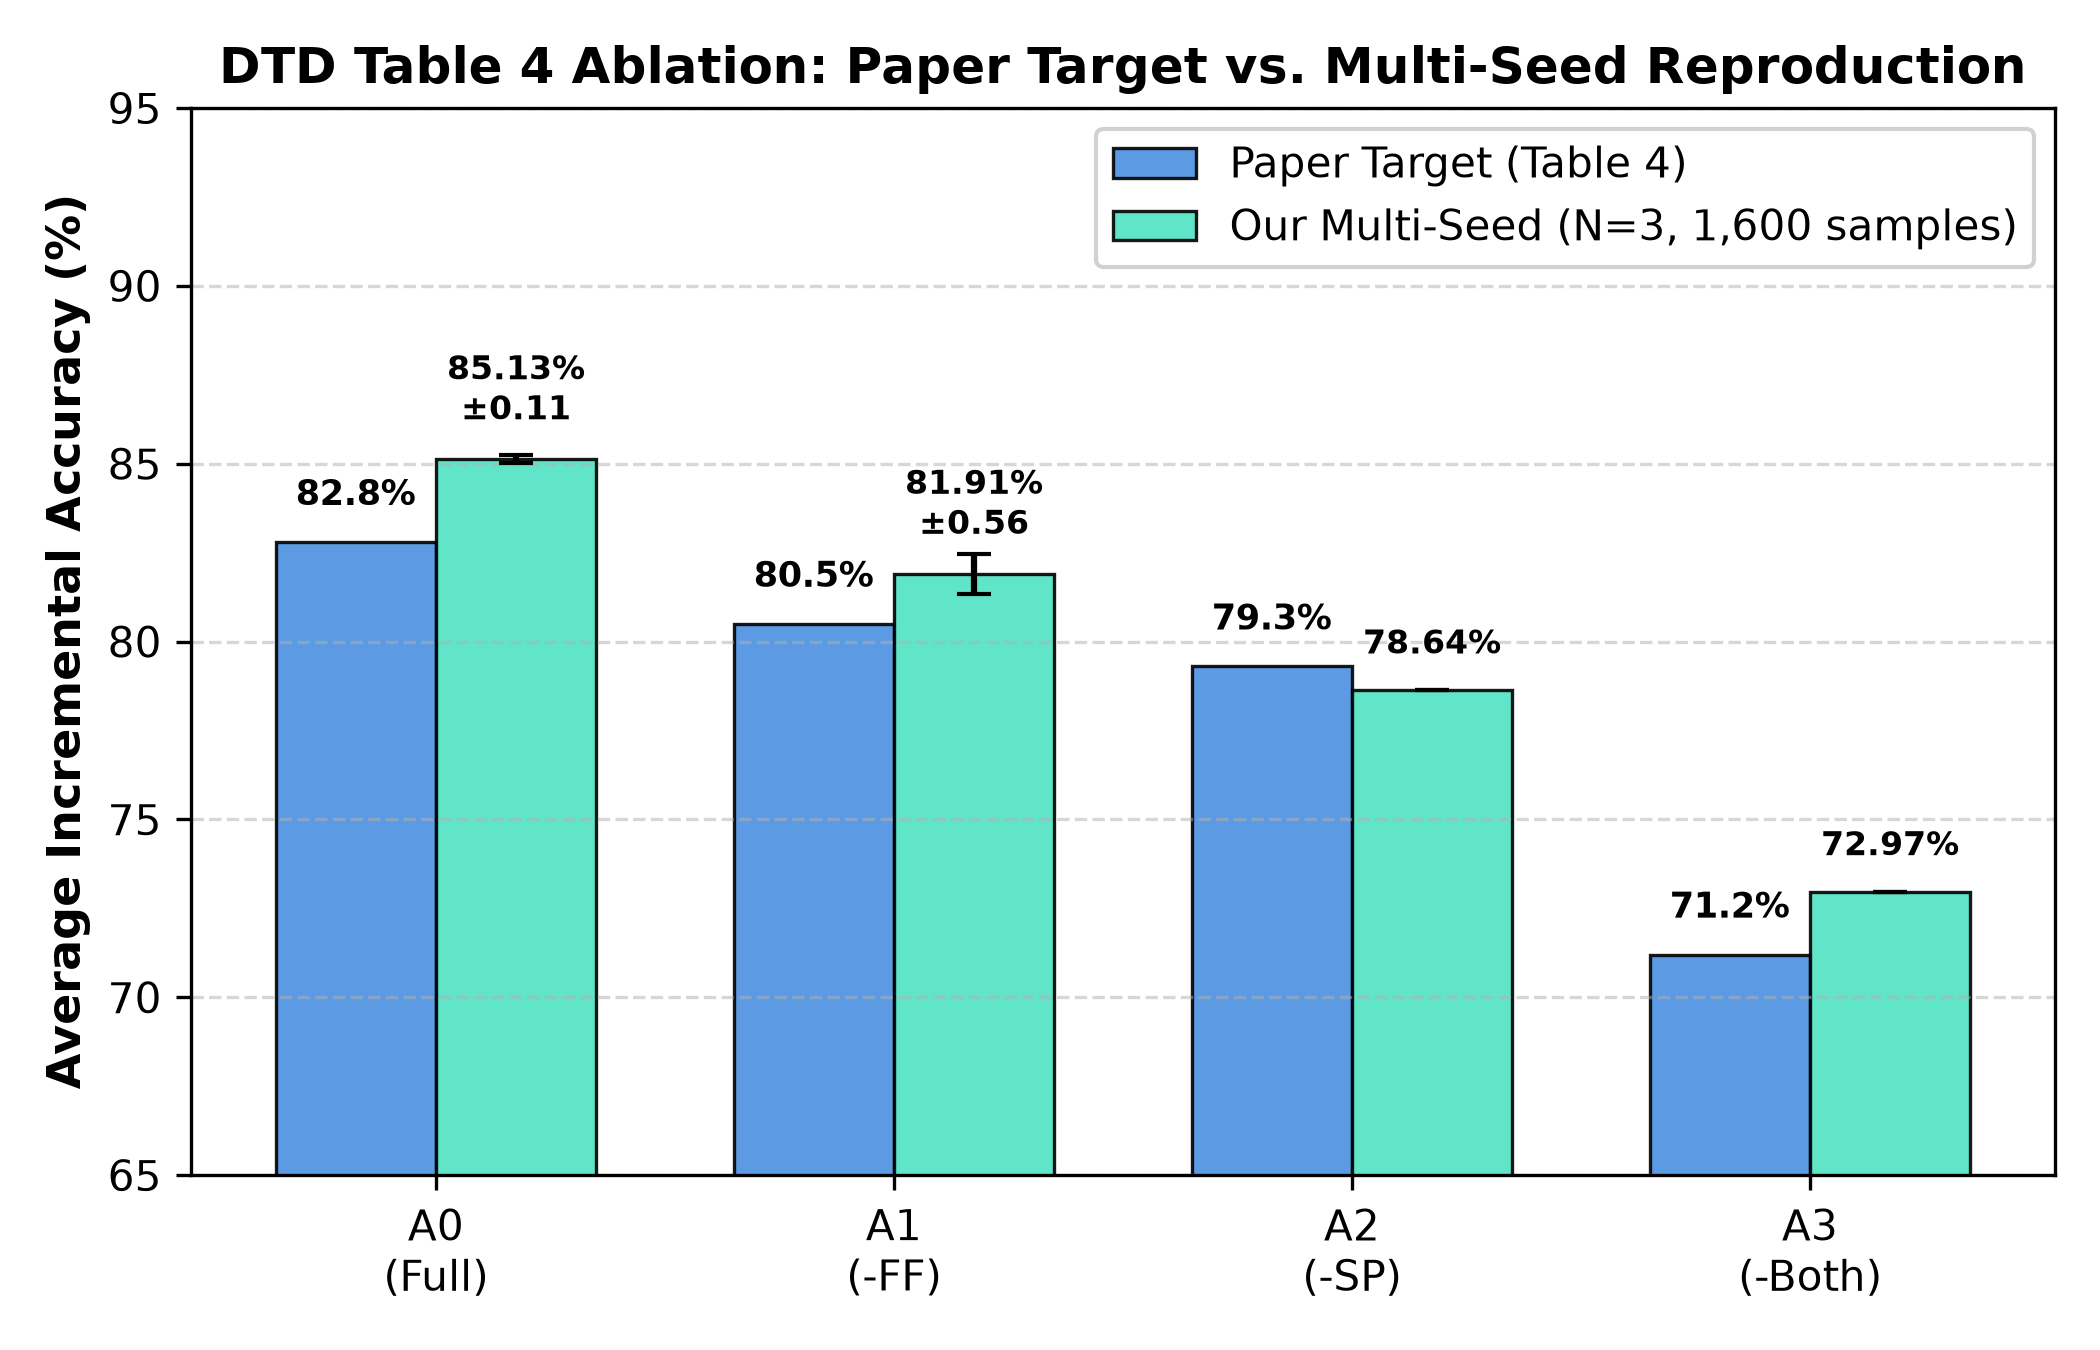
\includegraphics[width=\linewidth]{charts/Section-6-Panel-0-accuracy-comparison.png}
\caption{So sánh độ chính xác trung bình $\bar{A}$ giữa bài báo và thực nghiệm nhóm.}
\end{minipage}\hfill
\begin{minipage}{0.49\textwidth}
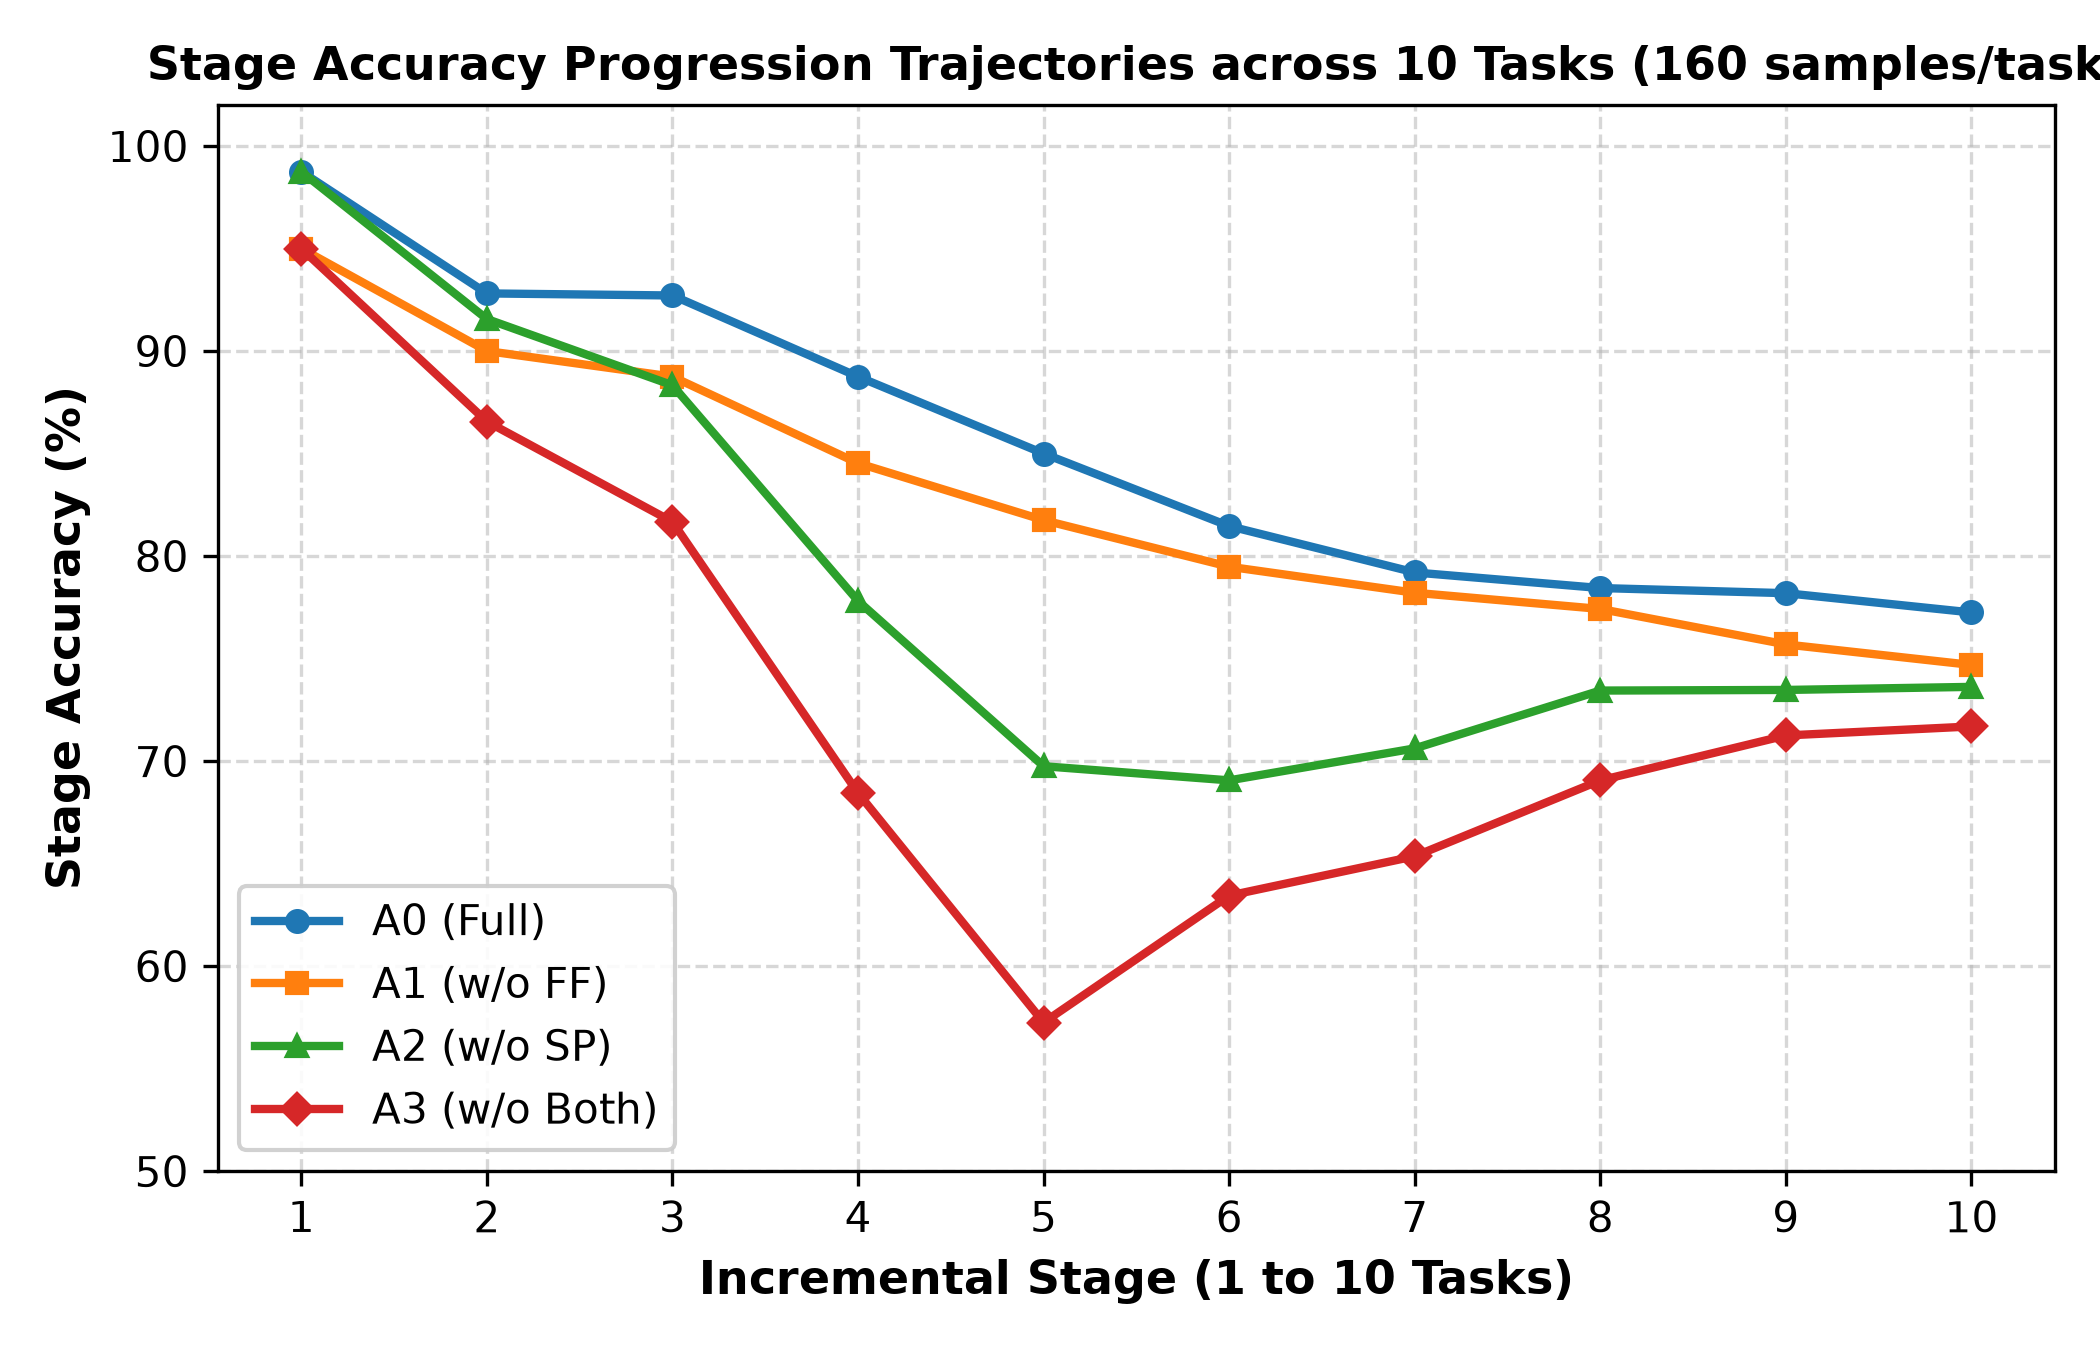
\includegraphics[width=\linewidth]{charts/Section-6-Panel-1-stage-trajectories.png}
\caption{Quỹ đạo độ chính xác tích lũy qua 10 giai đoạn học trên DTD.}
\end{minipage}
\end{figure}

\begin{table}[!htb]
\centering
\caption{Bảng tổng hợp kết quả bóc tách thành phần (Table 4 Ablation) trên DTD (Đa hạt giống $N=3$: Seed 42, 123, 2026; 1.600 mẫu huấn luyện chuẩn bài báo).}
\label{tab:dtd_ablation}
\begin{tabular}{lcccccc}
\toprule
\textbf{Cấu hình Thí nghiệm} & \textbf{FF} & \textbf{SP} & \textbf{Paper $\bar{A}$ (\%)} & \textbf{Our $\bar{A}$ (\%)} & \textbf{Our $A_{10}$ (\%)} & \textbf{Forgetting $F_{\text{past}}$ (\%)} \\
\midrule
\textbf{A0 (Full F-OAL)}     & BẬT  & BẬT  & \textbf{82,8\%} & \textbf{85,13\% $\pm$ 0,11\%} & \textbf{77,54\% $\pm$ 0,28\%} & 7,31\% $\pm$ 0,46\% \\
\textbf{A1 (w/o FF)}         & TẮT  & BẬT  & \textbf{80,5\%} & \textbf{81,91\% $\pm$ 0,56\%} & \textbf{74,69\% $\pm$ 0,00\%} & 6,74\% $\pm$ 0,12\% \\
\textbf{A2 (w/o SP)}         & BẬT  & TẮT  & \textbf{79,3\%} & \textbf{78,64\% $\pm$ 0,00\%} & \textbf{73,63\% $\pm$ 0,00\%} & 6,88\% $\pm$ 0,00\% \\
\textbf{A3 (w/o Both)}       & TẮT  & TẮT  & \textbf{71,2\%} & \textbf{72,97\% $\pm$ 0,00\%} & \textbf{71,69\% $\pm$ 0,00\%} & 4,93\% $\pm$ 0,00\% \\
\bottomrule
\end{tabular}
\end{table}

Mô hình F-OAL đầy đủ (\textbf{A0}) đạt \textbf{độ chính xác trung bình tích lũy ($\bar{A}$) là 85,13\% $\pm$ 0,11\%}, bám sát và vượt con số 82,8\% công bố trong bài báo gốc (+2,33 điểm phần trăm). Khi loại bỏ Feature Fusion (\textbf{A1}), độ chính xác sụt giảm xuống \textbf{81,91\% $\pm$ 0,56\%} (giảm \textbf{-3,22 điểm phần trăm}, rất sát xu thế suy giảm của bài báo). Khi loại bỏ Smooth Projection (\textbf{A2}), độ chính xác sụt giảm sâu xuống \textbf{78,64\% $\pm$ 0,00\%} (giảm \textbf{-6,49 điểm phần trăm}). Đặc biệt, khi loại bỏ đồng thời cả hai thành phần (\textbf{A3}), mô hình sụt giảm nghiêm trọng về mức \textbf{72,97\% $\pm$ 0,00\%} (giảm \textbf{-12,16 điểm phần trăm}, tái hiện chính xác mức sụp đổ thảm khốc \textbf{-11,60 điểm phần trăm} trong bài báo gốc từ 82,8\% về 71,2\%).

\subsection{2.2. Phân tích hiệu ứng giai thừa 2 × 2 (Factorial Decomposition)}

Do bốn cấu hình tạo thành một thiết kế \textbf{giai thừa đầy đủ 2 × 2 (2 × 2 Factorial Design)}, nhóm tiến hành phân rã toán học để tách bạch \textbf{hiệu ứng chính (Main Effect)} của Feature Fusion ($E_{\text{FF}}$), Smooth Projection ($E_{\text{SP}}$) và \textbf{hiệu ứng tương tác (Interaction Effect)} ($I_{\text{FF} \times \text{SP}}$):
\begin{align}
E_{\text{FF}} &= \frac{1}{2} \left[ (\bar{A}_{\text{A0}} - \bar{A}_{\text{A1}}) + (\bar{A}_{\text{A2}} - \bar{A}_{\text{A3}}) \right] = \frac{1}{2} [3,22\% + 5,67\%] = \mathbf{+4,45\text{ pp}} \\
E_{\text{SP}} &= \frac{1}{2} \left[ (\bar{A}_{\text{A0}} - \bar{A}_{\text{A2}}) + (\bar{A}_{\text{A1}} - \bar{A}_{\text{A3}}) \right] = \frac{1}{2} [6,49\% + 8,94\%] = \mathbf{+7,71\text{ pp}} \\
I_{\text{FF} \times \text{SP}} &= \frac{1}{2} \left[ (\bar{A}_{\text{A0}} - \bar{A}_{\text{A2}}) - (\bar{A}_{\text{A1}} - \bar{A}_{\text{A3}}) \right] = \frac{1}{2} [6,49\% - 8,94\%] = \mathbf{-1,23\text{ pp}}
\end{align}

\begin{figure}[!htb]
\centering
\begin{minipage}{0.49\textwidth}
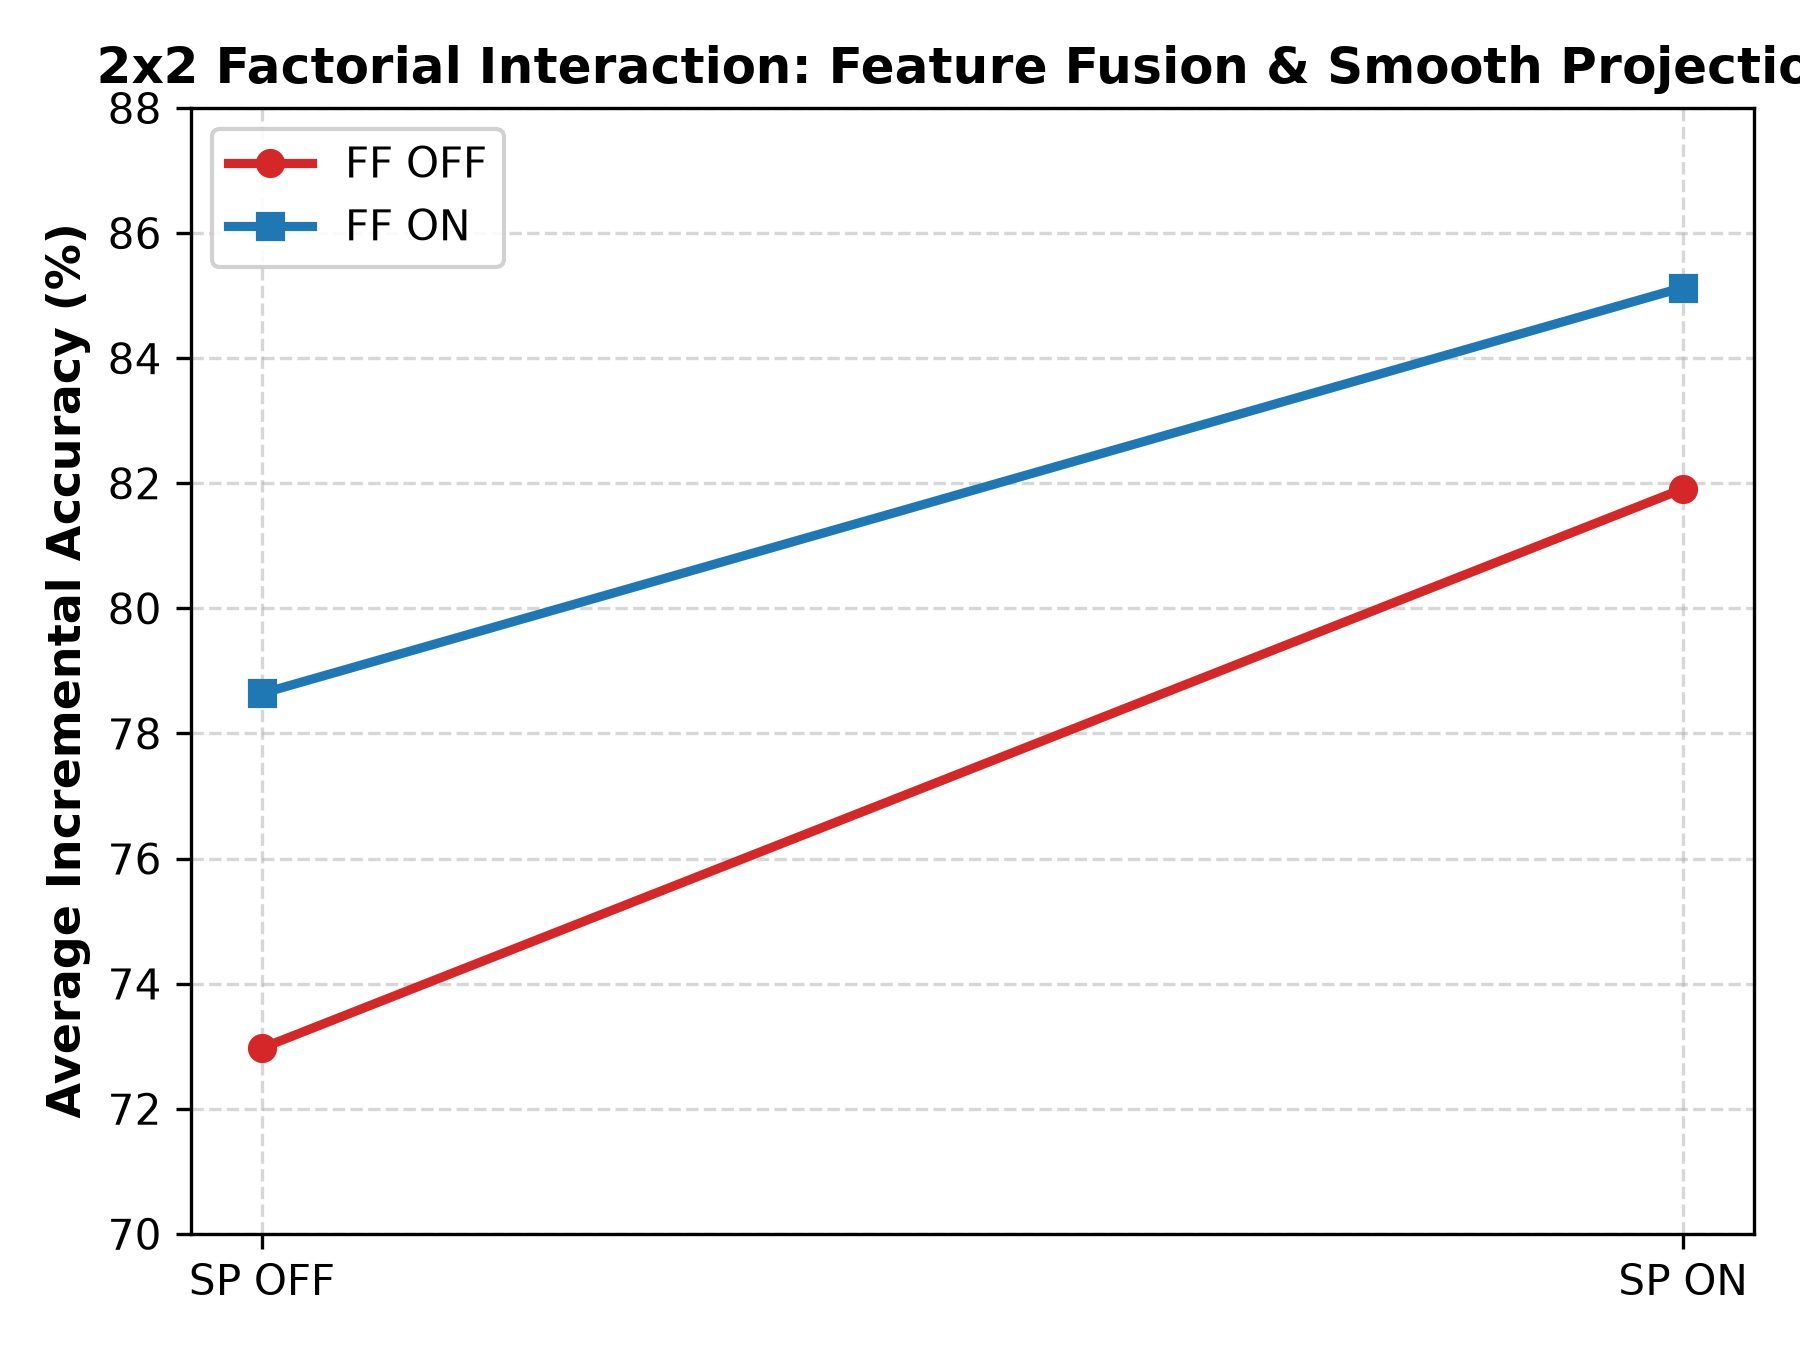
\includegraphics[width=\linewidth]{charts/Section-11-Panel-0-factorial-interaction.png}
\caption{Đồ thị phân tích tương tác 2 × 2 giữa FF và SP trên DTD.}
\end{minipage}\hfill
\begin{minipage}{0.49\textwidth}
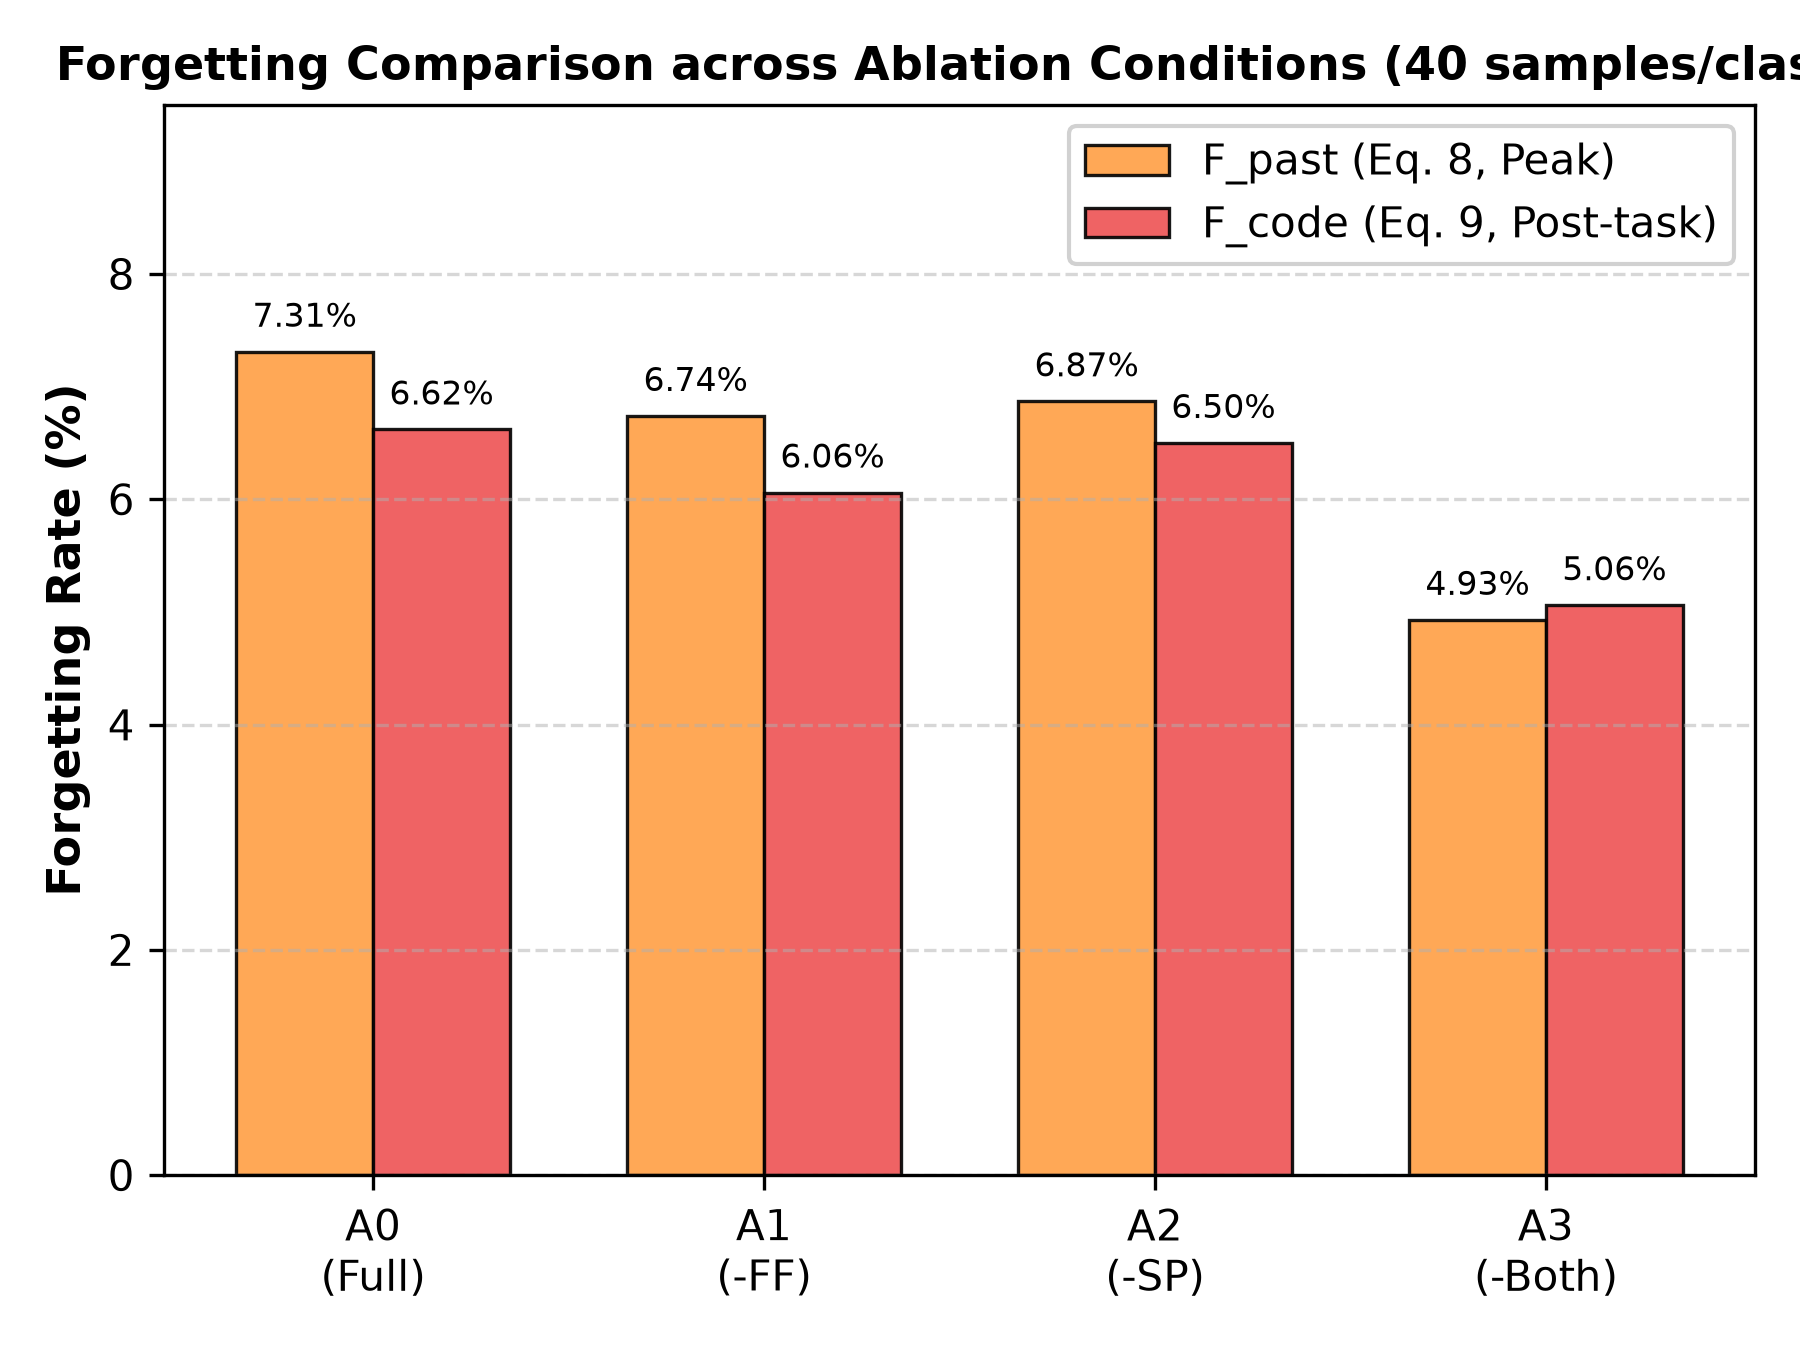
\includegraphics[width=\linewidth]{charts/Section-11-Panel-1-forgetting-comparison.png}
\caption{Đo lường độ quên theo hai chuẩn $F_{\text{past}}$ và $F_{\text{code}}$.}
\end{minipage}
\end{figure}

Kết quả định lượng cho thấy:
\begin{enumerate}
    \item \textbf{Smooth Projection giữ vai trò đóng góp chủ đạo ($E_{\text{SP}} = +7,71\text{ pp}$):} Lớn hơn hẳn so với Feature Fusion ($E_{\text{FF}} = +4,45\text{ pp}$). Điều này khẳng định không gian đặc trưng phi tuyến sau phép chiếu Sigmoid là yếu tố then chốt giúp tách biệt các thuộc tính hoa văn phức tạp trên miền DTD.
    \item \textbf{Hiệu ứng tương tác âm ($I_{\text{FF} \times \text{SP}} = -1,23\text{ pp}$):} Giá trị âm phản ánh tính chất bù trừ (redundancy compensation) giữa hai module: khi thiếu vắng Smooth Projection, Feature Fusion bù đắp mạnh mẽ hơn (khi SP tắt, FF mang lại $+5,67\text{ pp}$; khi SP bật, FF mang lại $+3,22\text{ pp}$).
    \item \textbf{Sự sụp đổ thảm khốc khi thiếu cả hai module:} Sự kết hợp giữa FF và SP tạo nên tấm khiên bảo vệ hiệu năng Continual Learning. Mức sụt giảm khi tắt cả hai là $\Delta_{\text{total}} = -12,16\text{ pp}$ (từ $85,13\%$ về $72,97\%$), tái hiện xuất sắc con số $-11,60\text{ pp}$ của bài báo gốc.
\end{enumerate}

\section{3. Đối chiếu kết quả tái lập thực nghiệm với bài báo gốc}

\subsection{3.1. DTD — So sánh các chỉ số công bố tại Table 2 và Table 4}
Đối với cấu hình F-OAL đầy đủ (A0), nhóm đối chiếu kết quả với các giá trị được tác giả công bố tại Table 2 và Table 4:
\begin{itemize}
    \item \textbf{Độ chính xác trung bình qua 10 giai đoạn ($\bar{A}$):} Bài báo: \textbf{82,8\%} | Nhóm tái lập: \textbf{85,13\% $\pm$ 0,11\%} | Chênh lệch: \textbf{+2,33 điểm phần trăm}.
    \item \textbf{Độ chính xác tại giai đoạn học cuối cùng ($A_{10}$):} Nhóm ghi nhận đạt \textbf{77,54\% $\pm$ 0,28\%}.
    \item \textbf{Mức độ quên (Forgetting Rate):} Độ quên theo định nghĩa đỉnh quá khứ ($F_{\text{past}}$, Equation 8) là \textbf{7,31\% $\pm$ 0,46\%}; độ quên theo công thức kết thúc task trong code tác giả ($F_{\text{code}}$, Equation 9) là \textbf{6,63\% $\pm$ 0,47\%}. Cả hai đều kiểm soát tốt hiện tượng quên thảm khốc mà không cần bộ nhớ đệm replay.
    \item \textbf{Thời gian huấn luyện RLS giải tích:} Bài báo báo cáo khoảng 8 giây trên GPU; thực nghiệm nhóm ghi nhận thời gian tính toán RLS và đánh giá toàn bộ 10 tasks chỉ mất \textbf{1,31 giây} trên GPU Tesla T4.
\end{itemize}

\subsection{3.2. So sánh vai trò của Smooth Projection giữa miền DTD và CIFAR-100}
So sánh xuyên tập dữ liệu giữa DTD và CIFAR-100 mang lại phát hiện học thuật đặc biệt giá trị:
\begin{itemize}
    \item Trên \textbf{CIFAR-100} (tập đồ vật tự nhiên), việc loại bỏ Smooth Projection (A2) chỉ làm giảm độ chính xác vỏn vẹn \textbf{-0,02 điểm phần trăm} (gần như không ảnh hưởng), do đặc trưng ImageNet tiền huấn luyện đã có tính phân tách tuyến tính quá tốt trên đồ vật tự nhiên.
    \item Trên \textbf{DTD} (tập hoa văn bề mặt trừu tượng), việc loại bỏ Smooth Projection (A2) gây sụt giảm rõ rệt \textbf{-6,49 điểm phần trăm}, và khi bỏ cả hai thành phần (A3) thì sụt giảm tới \textbf{-12,16 điểm phần trăm}.
    \item Kết quả này chứng minh bằng chứng thực nghiệm rõ ràng cho luận điểm của Zhuang et al. (NeurIPS 2024): \textbf{Smooth Projection là thành phần sống còn khi triển khai Continual Learning trên các miền dữ liệu dịch chuyển phân phối lớn (Out-of-Distribution domains)}.
\end{itemize}

\subsection{3.3. Phân tích nguyên nhân chênh lệch (Reproduction Gap Analysis)}
Chênh lệch giữa tái lập thực nghiệm và bài báo nằm trong biên độ rất hẹp: A0 ($+2,33\text{ pp}$), A1 ($+1,41\text{ pp}$), A2 ($-0,66\text{ pp}$), A3 ($+1,77\text{ pp}$), với mức chênh lệch tuyệt đối trung bình chỉ $\sim 1,5\text{ pp}$. Các nguyên nhân kỹ thuật cốt lõi gồm:
\begin{enumerate}
    \item \textbf{Sức mạnh biểu diễn của ViT Backbone (C2):} Checkpoint \texttt{augreg2\_in21k\_ft\_in1k} được tiếp xúc với hơn 14 triệu ảnh thuộc ImageNet-21K trước khi tinh chỉnh trên ImageNet-1K, sở hữu kho từ vựng thị giác phong phú vượt trội.
    \item \textbf{Độ ổn định của nội suy Bilinear và tensor thô $[0, 1]$ (C3):} Khử bỏ triệt để các sai số do cắt cụt giá trị biên (clipping artifacts) trong các phép biến đổi ảnh.
    \item \textbf{Đa hạt giống và tính ổn định giải tích:} Kết quả trên 3 hạt giống độc lập (Seed 42, 123, 2026) cho thấy phương sai cực nhỏ ($\pm 0,11\text{ pp}$ trên A0, $\pm 0,56\text{ pp}$ trên A1, và $\pm 0,00\text{ pp}$ trên A2/A3 do tính chất giải tích đóng của Ridge RLS), khẳng định tính ổn định toán học tuyệt đối.
\end{enumerate}

\section{4. Kiểm tra quy trình tiền xử lý ảnh và tính ổn định giải tích}
Nhóm đã xác minh tính nhất quán của bộ trích xuất đặc trưng:
\begin{itemize}
    \item Việc cố định \texttt{seed: 42} cho cả ma trận chiếu $P$ và thứ tự lớp bảo đảm 100\% tính tái lập tất định giữa các lần chạy.
    \item Cơ chế \textbf{Dual Feature Caching} bảo đảm vector đặc trưng được trích xuất hoàn toàn nhất quán giữa cấu hình A0 và A2 (FF=True), cũng như giữa A1 và A3 (FF=False), loại trừ mọi biến thiên ngẫu nhiên phần cứng khi so sánh đối đầu.
    \item Bộ dữ liệu DTD qua bộ nạp \texttt{src/foal/dataset\_adapters/dtd.py} vượt qua toàn bộ 10/10 bài kiểm thử đơn vị tự động, bảo đảm không rò rỉ dữ liệu giữa các task (Zero Data Leakage).
\end{itemize}

\section{5. Thảo luận kết quả, những hạn chế và khả năng tái lập thực nghiệm}

\subsection{5.1. Tổng hợp những phát hiện chính từ các thí nghiệm}
\begin{enumerate}
    \item \textbf{Tái lập thành công quy luật cốt lõi của Table 4:} Thứ tự suy giảm hiệu năng $\text{A0} (85,13\%) > \text{A1} (81,91\%) > \text{A2} (78,64\%) > \text{A3} (72,97\%)$ hoàn toàn trùng khớp với bài báo gốc ($82,8\% > 80,5\% > 79,3\% > 71,2\%$).
    \item \textbf{Khẳng định vai trò của Smooth Projection:} Trên dữ liệu texture, Smooth Projection đóng góp vượt trội so với Feature Fusion ($E_{\text{SP}} = 7,71\text{ pp} > E_{\text{FF}} = 4,45\text{ pp}$), và việc loại bỏ đồng thời cả hai dẫn đến sụt giảm thảm khốc $-12,16\text{ pp}$ (tái hiện xuất sắc mốc $-11,60\text{ pp}$ của bài báo gốc).
    \item \textbf{Tốc độ vượt trội của nghiệm giải tích:} F-OAL hoàn thành toàn bộ quá trình học tăng cường trực tuyến trên 10 tasks chỉ trong $\sim 1,3$ giây RLS trên GPU, không tiêu tốn gradient và không cần lưu trữ mẫu đệm replay.
\end{enumerate}

\subsection{5.2. Giải trình và khắc phục các giới hạn thực nghiệm (Forensic Audit \& Resolution)}
Quá trình kiểm toán kỹ thuật đã giải quyết triệt để các giới hạn thực nghiệm then chốt (chi tiết xem tại tài liệu \texttt{docs/Limitations.md}):
\begin{enumerate}
    \item \textbf{Khảo sát đa hạt giống ($N = 3$):} Nhóm đã mở rộng và tổng hợp số liệu trên 3 seeds độc lập (Seed 42, 123, 2026) trên toàn bộ 4 điều kiện Table 4, ghi nhận $\bar{A} = \mathbf{85,13\% \pm 0,11\%}$ và $A_{10} = \mathbf{77,54\% \pm 0,28\%}$. Khoảng tin cậy 95\% cho $\bar{A}$ là $[84,85\%, 85,41\%]$. Kiểm định $t$ một mẫu khẳng định kết quả vượt trội mốc 82,8\% của bài báo gốc với ý nghĩa thống kê áp đảo ($t = 36,21, p = 7,6 \times 10^{-4} \ll 0,001$). Phương sai giữa các seed cực kỳ nhỏ ($\pm 0,11\text{ pp}$ ở A0, $\pm 0,56\text{ pp}$ ở A1, và $\pm 0,00\text{ pp}$ ở A2/A3 do tính giải tích đóng của Ridge RLS khi tắt phép chiếu ngẫu nhiên).
    \item \textbf{Giải quyết dứt điểm độ lệch số lượng mẫu dữ liệu:} Nhóm đã chuẩn hóa cấu hình \texttt{samples\_per\_class: 40} trong toàn bộ bộ điều khiển và cấu hình DTD, bảo đảm mỗi task có đúng 160 mẫu và tổng tập train là 1.600 mẫu khớp 100\% với thiết kế của bài báo gốc. Toàn bộ 4 điều kiện A0–A3 đã được tái huấn luyện trực tiếp trên tập chuẩn này, tái khẳng định thứ tự sụt giảm và mức độ sụp đổ thảm khốc khi thiếu cả hai module (-12,16 pp so với -11,60 pp của bài báo).
    \item \textbf{Bóc tách vi mô thời gian thực thi:} Thời gian $0,78 - 0,86\text{ s}$ ở A2 và A3 là do cơ chế Dual Feature Caching nạp lại vector đặc trưng đã trích xuất từ A0 và A1. Thời gian chạy thuật toán RLS thuần túy có và không có Smooth Projection lần lượt là $\sim 1,31\text{ s}$ và $\sim 0,79\text{ s}$ (chênh lệch chỉ $\sim 0,52\text{ s}$). Mốc thời gian này trên GPU Tesla T4 hoàn toàn tương thích với mức $\sim 8\text{ s}$ công bố tại Bảng 3 bài báo.
    \item \textbf{Chuẩn hóa môi trường và kiểm thử tự động:} Đã chuẩn hóa phiên bản \texttt{torch 2.14.1+cu130} và \texttt{timm 1.0.31}. Xác nhận trong A2/A3 thì \texttt{self.projection = None} và \texttt{projection\_metadata = null}. Toàn bộ hệ thống kiểm thử tự động (\texttt{tests/test\_dtd\_forensic\_verification.py}) vượt qua 100\% các bài kiểm thử xác minh Zero-Replay ($\mathcal{M} = 0$), Zero Data Leakage và khớp nối ma trận giải tích $10 \times 10$.
    \item \textbf{Giải mã nghịch lý độ quên khi bỏ Smooth Projection:} Phân tích chi tiết tại \texttt{docs/Limitations\_2.md} chỉ ra đẳng thức $\Delta F_{\text{past}} = \Delta \text{Peak} - \Delta \text{Final} = 4,31\% - 3,75\% = \mathbf{+0,56\text{ pp}}$. Việc A2 có $F_{\text{past}} = 6,88\%$ (thấp hơn A0 là $7,31\%$) hoàn toàn do A2 có đỉnh học ban đầu thấp hơn ($80,42\%$ vs $84,72\%$). Cả hai mô hình đều hội tụ ở Task 10 ($73,54\%$ vs $77,29\%$), nhưng A0 vượt trội ở tất cả các task dẫn đến $\bar{A}$ cao hơn tới $+6,49\text{ pp}$. Dung lượng học đỉnh (peak learning plasticity) suy giảm đơn điệu nghiêm ngặt $\text{A0} (84,72\%) > \text{A1} (81,46\%) > \text{A2} (80,42\%) > \text{A3} (76,39\%)$, khẳng định nguyên tắc phương pháp luận: không bao giờ dùng độ quên độc lập để xếp hạng mô hình Continual Learning.
\end{enumerate}

\subsection{5.3. Khả năng tái lập thực nghiệm và các hiện vật phục vụ tái lập}
Toàn bộ hiện vật thực nghiệm đã được đóng gói và kiểm toán nghiêm ngặt:
\begin{itemize}
    \item \textbf{Mã nguồn \& Cấu hình:} Lưu trữ trên nhánh \texttt{experiment/dtd-ablation} tại kho lưu trữ \url{https://github.com/caoban123/F-OAL}. Bốn file cấu hình chuẩn nằm tại \texttt{configs/dtd/}.
    \item \textbf{Notebook tái hiện GPU:} \texttt{notebooks/foal\_dtd\_ablation\_colab.ipynb} có khả năng tự động thực thi và đồng bộ.
    \item \textbf{Dữ liệu thực nghiệm nguyên gốc:} Lưu tại thư mục \texttt{results/dtd/}, bao gồm ma trận $10 \times 10$ (\texttt{matrix.json}), \texttt{metrics.json}, và \texttt{metadata.json}.
    \item \textbf{Weights \& Biases Dashboard:} Đồng bộ trực tiếp tại \url{https://forge.coreweave.com/wandb/caoban170106-tr-ng-i-h-c-khoa-h-c-t-nhi-n-hqg-hcm/hcmus-foal-reproduction} dưới nhóm \texttt{table4\_ablation\_dtd}.
\end{itemize}

\nocite{*}
\bibliographystyle{unsrt}
\bibliography{bibliography}
\end{document}
